\documentclass{beamer}
 
\usepackage[utf8]{inputenc}
\usepackage{listings}

\lstdefinestyle{consola}
	{basicstyle=\scriptsize\bf\ttfamily,
	backgroundcolor=\color{gray}}
\lstdefinestyle{Python}
	{language=Python}
	
% https://www.sharelatex.com/learn/Beamer
% % https://learnxinyminutes.com/docs/julia/
%Information to be included in the title page:
\title{Introducción al lenguaje Julia}
\author{
\includegraphics[scale=0.5]{images/128px-Julia_prog_language}\\Francisco Gárate}
%\author{Francisco Gárate \\\texttt{paco@garpa.net}}
\institute{Jornadas Medialab-Prado}
\date{13-14, febrero 2018}

\definecolor{azul_w}{RGB}{66,103,213}
\definecolor{verde_w}{RGB}{60,151,46}
\definecolor{rojo_w}{RGB}{201,61,56}
\definecolor{morado_w}{RGB}{148,91,176}
\setbeamercolor{title}{bg=azul_w,fg=white}
\setbeamercolor{frametitle}{fg=verde_w}
\setbeamercolor{structure}{fg=rojo_w}
% \setbeamercolor{title}{fg=red!80!black,bg=red!20!white}

\logo{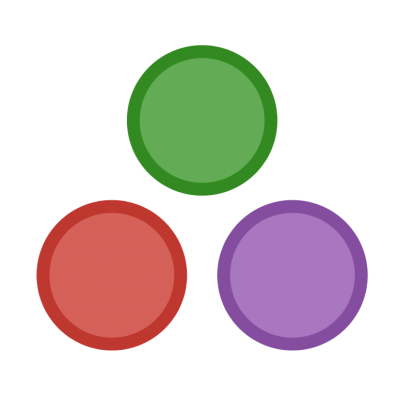
\includegraphics[scale=0.10]{images/logo}\vspace{220pt}}

\providecommand{\comando}[1]{\texttt{\colorbox{morado_w}{\textcolor{white}{#1}}}}

\begin{document}
\frame{\titlepage}
 
\begin{frame}
\frametitle{¿Quién es Julia?}
\begin{itemize}
	\item Julia es un lenguaje de programación libre, de código abierto (licencia MIT) y con librerías amigables.
	\item Creado en el MIT por Jeff Bezanson, Alan Edelman, Stefan Karpinski y Viral Shah en 2009, y publicado en 2012.
	\item Diseñado especialmente para entornos científicos y matemáticos. 
	\item \textit{"Walks like Python. Runs like C"}. Se lee igual que Python o Octave, pero se comporta casi igual de rápido que C.
	\item Lenguaje diseñado para correr en paralelo y en la nube fácilmente.
	\item Documentación: \url{https://docs.julialang.org}
\end{itemize}
\end{frame}

\begin{frame}
\frametitle{Instalar Julia}
\begin{itemize}
	\item Descargar instalador: \url{http://julialang.org/downloads/}
	\item En linux: \comando{apt-get install julia}
	\item Julia incluye un terminal interactivo llamado REPL:
		\begin{itemize}
		\item \comando{;} La siguiente instrucción se ejecuta como si fuera una consola de linux
		\item \comando{?} Busca el texto a introducir en los manuales de ayuda
		\end{itemize}
\end{itemize}
\begin{center}
	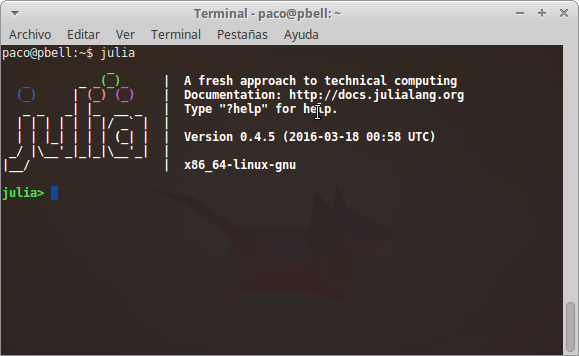
\includegraphics[scale=0.35]{images/julia-consola}
\end{center}
\end{frame}

\begin{frame}
\frametitle{IDE}
\begin{itemize}
	\item Soporte para: Vi(m), emacs, Eclipse, Sublime Text...
	\item Recomendación: Atom + Juno (\url{http://junolab.org})
	%\item desde Atom: '\texttt{Ctrl ,}' o '\texttt{Cmd ,}' -  Install - 'uber juno'
\end{itemize}
\begin{center}
	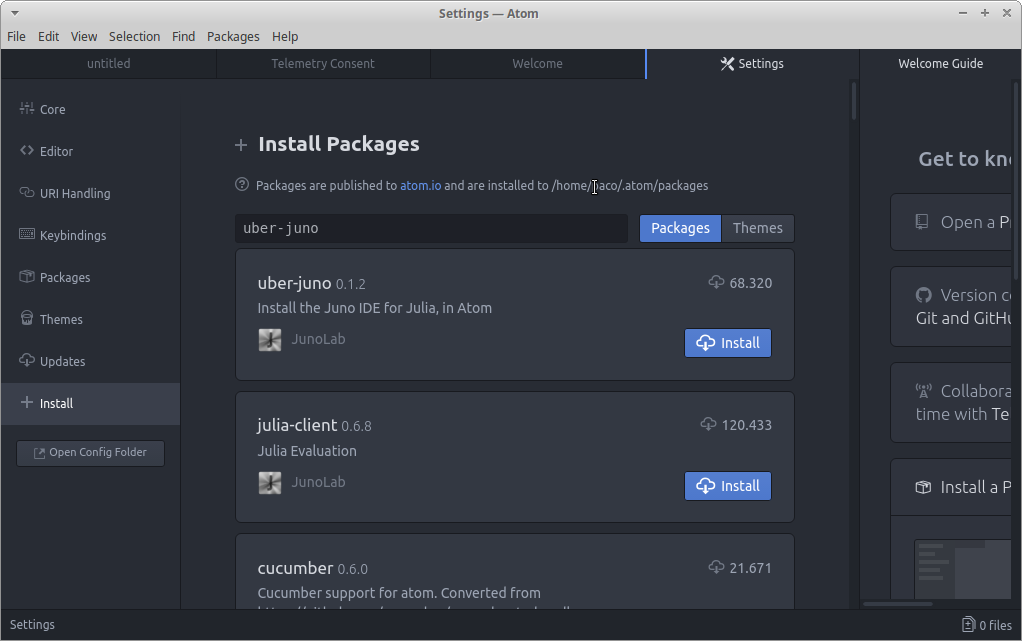
\includegraphics[scale=0.20]{images/atom-juno}\\
	\small{desde Atom: \comando{Ctrl ,} o \comando{Cmd ,},  Install, 'uber-juno'}
\end{center}
\end{frame}

\begin{frame}
\frametitle{Prueba Julia (sin instalar)}
\begin{itemize}
	\item Jupyter Notebook: IJulia (similar a IPython): \url{https://try.jupyter.org}
	\item \texttt{www.juliabox.com} Incluye +100 paquetes
\end{itemize}
\begin{center}
	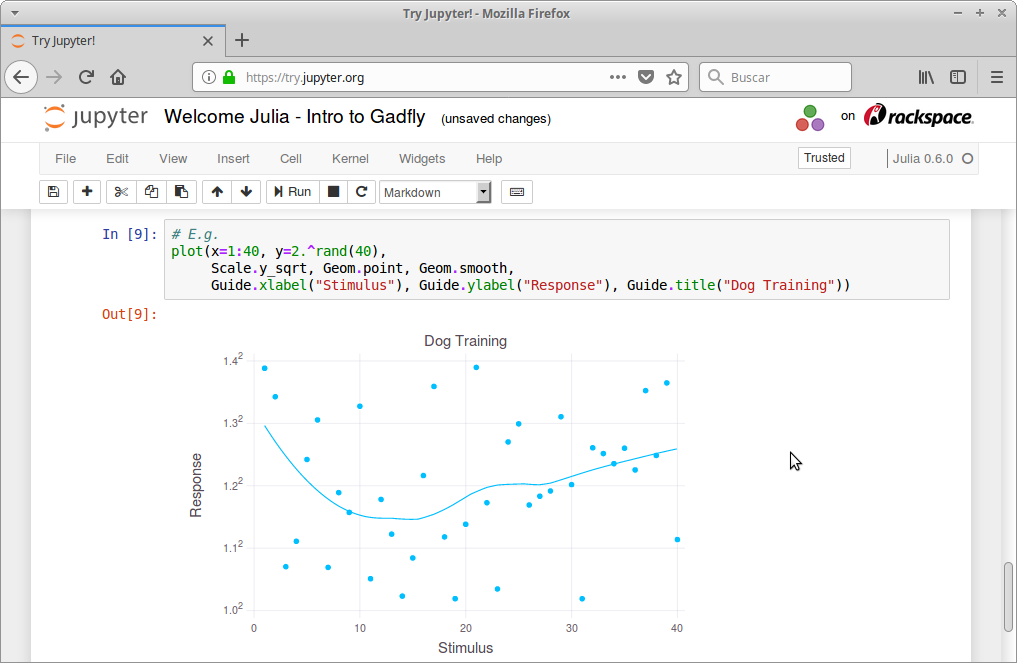
\includegraphics[scale=0.25]{images/jupyter-julia}
\end{center}
\end{frame}

\begin{frame}
\frametitle{Paquetes (Packages)}
\begin{itemize}
	\item Repositorio oficial: \url{http://pkg.julialang.org}
	\item Existen actualmente 1.703 paquetes registrados y testeados: \url{http://pkg.julialang.org/pulse.html}
	\item Para instalar: \comando{Pkg.add("Distributions")}
	\item Desinstalar: \comando{Pkg.rm("Distributions")}
	\item Para ver el estado de tus paquetes: \comando{Pkg.status()}
\end{itemize}
\end{frame}

\begin{frame}{Hola Mundo}
\begin{itemize}
	\item \texttt{println("Hola Mundo")}
	\item Desde shell: \comando{julia holamundo.jl}
	\item Operadores \texttt{+, -, *, /}\\
	\texttt{a = 4.0}\\
	\texttt{b = 7.0}\\
	\texttt{c = (b - a) * (b + a) / a}
	\item Funciones matemáticas familiares:\\
	\texttt{result = exp(-2.33) * cos(22 * 180 / pi)}
	\item Funciones incluidas de serie. Por ejemplo:\\
	\texttt{rand()} \textit{(genera números aleatorios entre 0 y 1)}\\
	\texttt{std(v)/mean(v)}
	\item Condicionales, listas, loops, rangos, etc.. al estilo Python
\end{itemize}
\end{frame}

\begin{frame}
\frametitle{¿Por qué Julia?}
\begin{center}
Teniendo R, Matlab, Mathematica, Python...\\
¿De verdad hace falta otro lenguaje de programación?\\[0.5cm]

\includegraphics{images/1316694066614.jpg}	
\end{center}
\end{frame}

\begin{frame}
\frametitle{¿Por qué Julia?}
\begin{itemize}
	\item Julia no es popular. 
	\item No aparece en el ranking de los lenguajes más populares de GitHub \footnotemark ni en el Top 20 Most Popular de Stackoverflow\footnotemark.
	\item Tampoco la NASA\footnotemark  o el CERN han liberado ninguna librería (de momento).
	\item ... pero eso también mola!
	\item Veamos las ventajas de Julia frente a otros lenguajes:
\end{itemize}
\end{frame}

\begin{frame}
\frametitle{Ventajas}
\framesubtitle{Soporte Unicode}
\begin{itemize}
	\item Se introducen símbolos al igual que \LaTeX
\end{itemize}
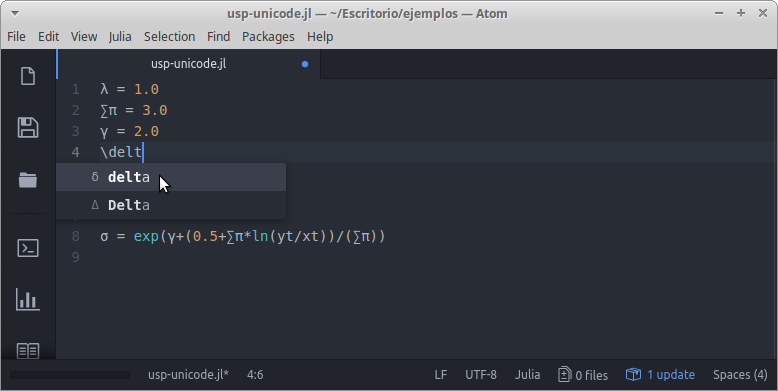
\includegraphics[scale=0.40]{images/julia-unicode}
\end{frame}


\begin{frame}
\frametitle{Ventajas}
\framesubtitle{Compilador JIT}
\begin{itemize}
	\item Su compilador JIT (Just-In-Time) basado en LLVM (Máquina Virtual de Bajo Nivel) permite a Julia acercarse, e incluso igualar, a C.\\
	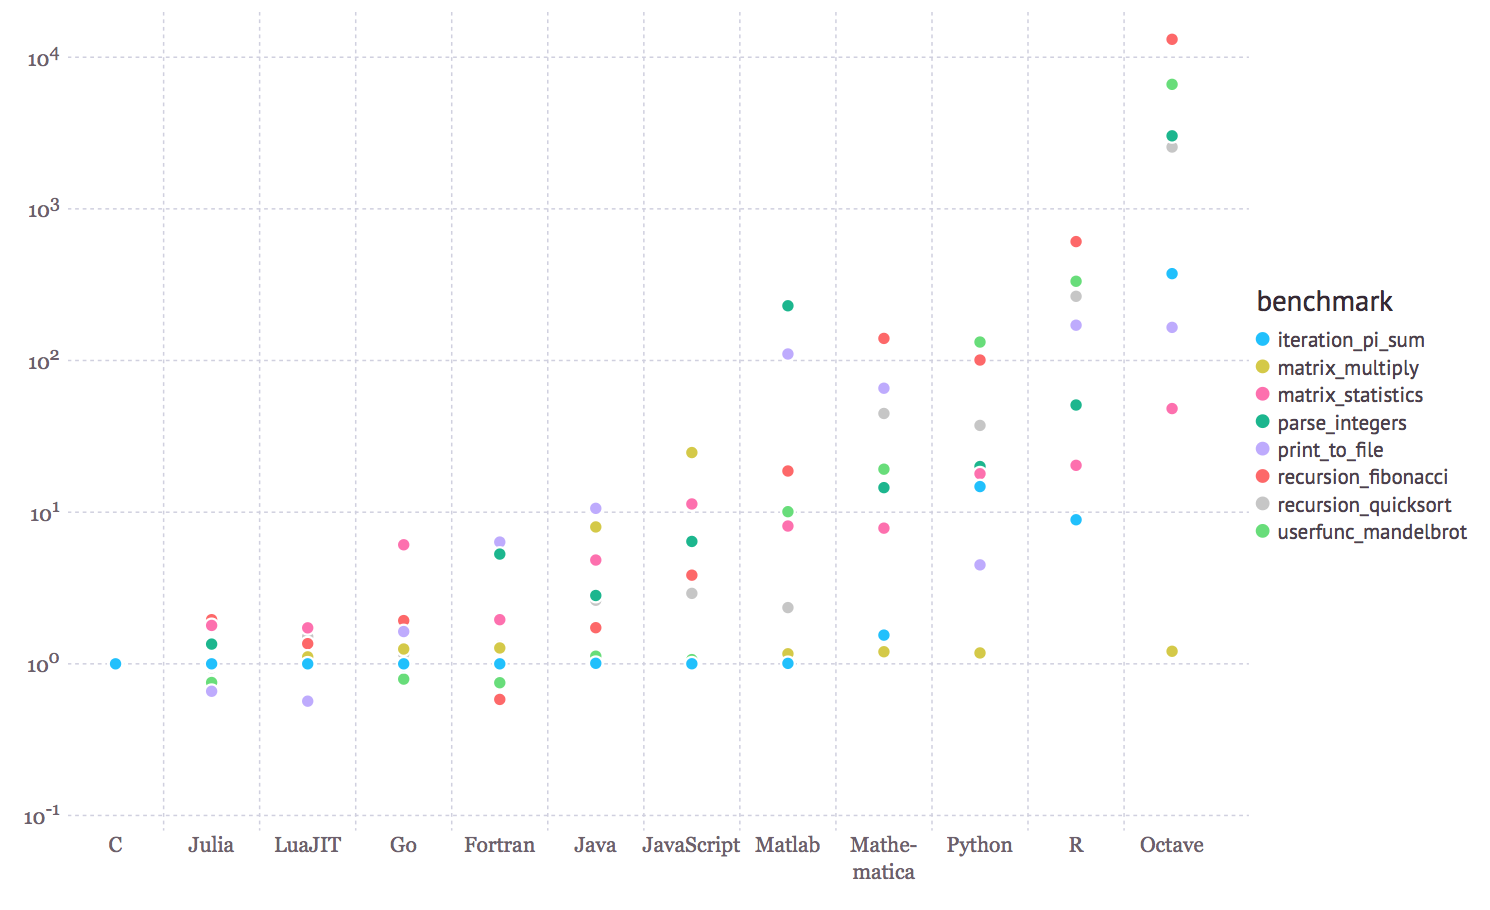
\includegraphics[scale=0.35]{images/benchmarking-julia}
\end{itemize}
\end{frame}

\begin{frame}
\frametitle{Ventajas}
\framesubtitle{Computación en paralelo de forma nativa}
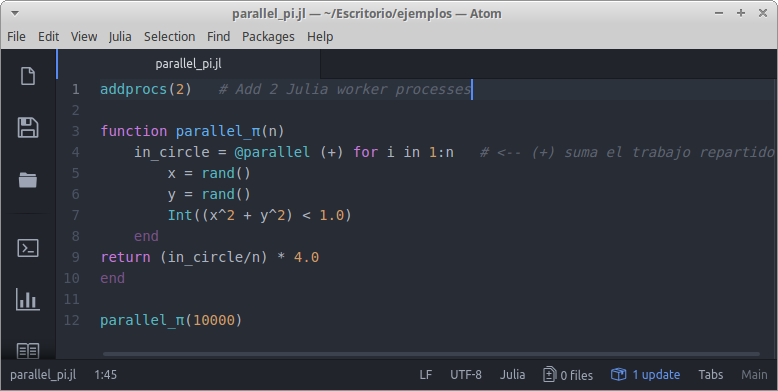
\includegraphics[scale=0.37]{images/julia-pararell-pi}
\begin{itemize}
	\item Repositorio de modelos para programación en paralelo: \url{https://juliaparallel.github.io}
	\item Celeste.jl\footnotemark: Librería que ha incrementado x225 la velocidad del análisis de imágenes (dataset de 55 TB) ayudando al NERSC en la catalogación de objetos astronómicos
\end{itemize}
\end{frame}


\begin{frame}
\frametitle{Ventajas}
\framesubtitle{Otras razones}
\begin{itemize}
	\item Licencia MIT (compatible con GNU GPL)
	\item Robusto ecosistema de herramientas estadísticas, distribución en paralela, optimización y de visualización de datos.
	\item Librerías gráficas (como Gadfly) para jugar en primera división.
	\item Llamadas a librerías C, Fortran de forma nativa:\\
	\comando{julia$>$ccall(:clock, Int32, ())}\\
	1180595\\
	\item ...y a Python (a través de PyCall.jl)
	\item Sintaxis familiares a Python
	\item En resumen: Unir facilidad de uso y alto rendimiento es posible.
\end{itemize}
\end{frame}


\begin{frame}
\frametitle{\#JuliaLangEs}
\begin{itemize}
	\item Se buscan voluntarios para:
	\begin{itemize}
		\item Dar a conocer el lenguaje Julia 
		\item Traducir la documentación oficial al castellano
		\item Crear/Potenciar una comunidad de usuarios de Julia en español (blog, meetup, etc...)
		\item Crear o migrar librerías de R/Python a Julia
	\end{itemize}
	\item Mas info: paco@garpa.net o
	\begin{itemize}
	\item \url{https://github.com/franciscogarate/Introduccion-al-lenguaje-Julia}
	\end{itemize}
\end{itemize}
\end{frame}

\begin{frame}
\frametitle{Referencias}
\begin{itemize}
	\item [1]{\url{https://octoverse.github.com}}
	\item [2]{\url{https://insights.stackoverflow.com/survey/2017\#technology}}
	\item [3]{\url{https://code.nasa.gov/?q=julia} \textit{(consulta vacía)}}
	\item [4]{\url{https://juliacomputing.com/press/2016/11/28/celeste.html}}
\end{itemize}
\end{frame}




\end{document}